\begin{figure}[H]
    \centering
    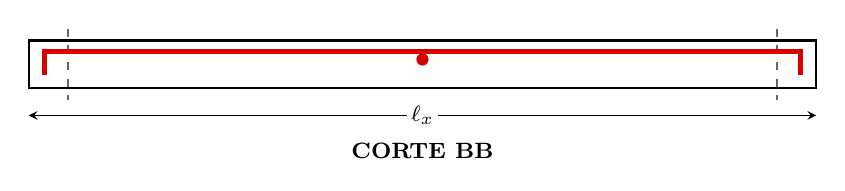
\begin{tikzpicture}[
        scale=1,
        >=stealth,
        contorno/.style={draw=black, thick},
        margem/.style={draw=gray!80!black, thick},
        barra/.style={line width=1.6pt, red!85!black},
        chamada/.style={gray!60!black, thin, dashed},
        cota/.style={<->, thin, black},
        corte/.style={draw=black, dash dot, thick},
        setaCorte/.style={->, very thick, black},
        txt/.style={font=\footnotesize\bfseries, inner sep=1.5pt}
    ]

    % ---------- Parâmetros (planta) ----------
    \def\W{10}      % largura do retângulo maior
    \def\H{6.5}     % altura do retângulo maior (menor que \W)
    \def\m{0.5}     % distância entre os retângulos (= 20 em x e y)
    \def\ext{0.3}   % quanto a barra sai do retângulo menor (< \m)
    \pgfmathsetmacro\cx{\W/2}
    \pgfmathsetmacro\cy{\H/2}

    %\node[txt] at (\cx,-1.2) {PLANTA DA LAJE};

    % ========== 2. CORTE BB (largura = \W) ==========
    \def\t{0.6}      % espessura da laje no desenho
    \def\dl{0.14}    % posição da armadura (d')
    \def\gh{0.3}     % gancho
    \def\yTop{-2.2}  % topo da laje no corte BB

    \draw[contorno] (0,\yTop) rectangle (\W,\yTop-\t);
    \draw[margem, dashed] (\m,\yTop+0.15) -- (\m,\yTop-\t-0.15);
    \draw[margem, dashed] (\W-\m,\yTop+0.15) -- (\W-\m,\yTop-\t-0.15);
    % barra principal em comprimento (ganchos para baixo)
    \draw[barra] (\m-\ext,\yTop-\dl-\gh) -- (\m-\ext,\yTop-\dl)
                 -- (\W-\m+\ext,\yTop-\dl) -- (\W-\m+\ext,\yTop-\dl-\gh);
    % barra secundária em ponto
    \fill[red!85!black] (\cx,\yTop-\dl-0.1) circle (2.2pt);
    \draw[cota] (0,\yTop-\t-0.35) -- (\W,\yTop-\t-0.35)
        node[midway, fill=white, txt] {$\ell_x$};
    \node[txt] at (\cx,\yTop-\t-0.8) {CORTE BB};

    \end{tikzpicture}
    %\caption{Planta da laje e cortes AA e BB}
\end{figure}